\documentclass[a4paper,11pt,article,oneside]{memoir}
\usepackage{ecis2023}


%%% About this LaTeX template: %%%%%%%%%%%%%%%%%%%%%%%%%%%%%%%%%%%%%%%%%%%%%%%
%
% This template should work with any (reasonably recent) full
% installation of TeXLive or MikTeX. The "ecis2023" package loads a
% number of other packages, so if some package is missing, please
% install it using the package manager of your TeX distribution. In
% particular, if the "tikz" package is missing, you may have to install
% "pgf" or simply remove our example graphics (see figure example
% below).
%
% The file "ecis2023.sty" should be placed somewhere in your TeX Path
% (or simply in the same folder as your document).
%
% Please use PDFLaTeX to compile your document.
%
% You need not escape special characters or Umlauts like é ä ö ü ß (in 
% fact, you shouldn't), as this source is inputenc'd in UTF-8.
%
% Note for BibTeX users: We use BibLaTeX for formatting, so we use Biber
% as a sorting backend (default). 
% If you still need to use the old BibTeX program, please change the 
% BibLaTeX backend in the package file ("ecis2023.sty").
%
% The ERCIS 2023 template is based on the one created for ECIS 2019.
% Adapted for ECIS 2023 by Tim A. Majchrzak.
%
% Greetings to all Information Systems researchers using LaTeX!
%
%%% Enter Document Info here: %%%%%%%%%%%%%%%%%%%%%%%%%%%%%%%%%%%%%%%%%%%%%%%%

\maintitle{Application of Microservices Patterns to Big Data Systems} % ← Don't use UPPERCASE here, we do that automatically.
\shorttitle{Big Data and Microservices} % ← This goes into the header.
\category{Complete Research} % ← Choose one by deleting the others.

% The review process is double blind.
% Therefore papers submitted for review MUST NOT contain any author 
% information – neither on the title page nor in the page header! 
% This information will be added only once the submission is ACCEPTED.

%\authors{% Separate authors by a "\par" or blank line.
%Smith, Ellen, University of Trinithlon, Trinithlon, UK, ellen.smith@utri.ac.uk

%Jönsson, Mikael, University of Oxenhagen, Oxenhagen, Sweden, mikael.jonsson@inf.uox.se}

%\shortauthors{Example et al.} % ← This goes into the header. 

%%% BibTeX: %%%%%%%%%%%%%%%%%%%%%%%%%%%%%%%%%%%%%%%%%%%%%%%%%%%%%%%%%%%%%%%%%%

\addbibresource{references.bib} % ← Your .bib file, if you're using BibTeX

%%%%%%%%%%%%%%%%%%%%%%%%%%%%%%%%%%%%%%%%%%%%%%%%%%%%%%%%%%%%%%%%%%%%%%%%%%%%%%
%%%%%%%%%%%%%%%%%%%%%%%%%%%%%%%%%%%%%%%%%%%%%%%%%%%%%%%%%%%%%%%%%%%%%%%%%%%%%%

\begin{document}

\noindent\fbox{%
	\parbox{\textwidth}{%
		\hfill{}
		\vspace{10em}
	}%
}

\begin{abstract}\noindent
    The panorama of data is ever evolving, and big data has emerged to become one of the most hyped terms in the industry. Today, users are the perpetual producers of data that if gleaned and crunched, will yield game-changing patterns. This has introduced an important shift about the role of data in organizations and many strived to harness to power of this new material. Howbeit, institutionalizing data is not an easy task and requires the absorption of a great deal of complexity. According to a recent survey, it is estimated that only 13\% of organizations succeeded in delivering on their data strategy. Among the root challenges, big data system development and data architecture are prominent. To this end, this study aims to facilitate data architecture and big data system development by applying well-established patterns of microservices architecture to big data systems. This objective is achieved by two systematic literature reviews, and infusion of results through thematic synthesis. The result of this work is a series of theories that explicates how microservices patterns could be useful for big data systems. These theories are then validated through a semi-structured interview with 7 experts from the industry. The findings emerged from this study indicates that big data architecture can benefit from many principles and patterns of microservices architecture. 
\end{abstract}

\begin{keywords}
    big data, microservices, microservices patterns, big data architecture, data architecture, data engineering
\end{keywords}

% NOTE: Important information
%1.	Completed research papers are limited to a maximum of thirteen (13) pages. The page limit includes all text (including title, abstract, keywords), figures, tables, and appendices. The references are excluded from this page count.
%2.	Start the main body of the paper (i.e., the Introduction section) on the FIRST page; that is, right after the Abstract/Keywords.
%3.	Submission files must be in PDF format.


\chapter{Introduction}


Today, we live in a world that produces data at an unprecedented rate. The attention toward these large volume of data has been growing rapidly and many strive to harness the advantages of this new material. While the opportunities exist with big data (BD), there are many failed attempts. According to \citet{NewVantageSurvey} in 2022, only 26.5\% of companies successfully became data-driven. Another survey by \citet{DataBricksSurvey} highlighted that only 13\% of organizations succeeded in delivering on their data strategy. Among the challenges of adopting BD, data architecture, organizational culture, lack of talent, and rapid technology change are bold. 

Therefore, there is an increasing need for more research on reducing the complexity involved with BD projects. One area with good potential is data architecture. Data architecture allows for a flexible and scalable BD system that can account for emerging requirements. One concept that has the potential to help with development of BD systems is the use of microservices (MS) architecture. MS architecture allows for division of complex applications into small, independent, and highly scalable parts and, therefore, increases maintainability and allows for a more flexible implementation \citep[p.~20]{Richardson.2022}. Nevertheless, design and development of MS is sophisticated, since heterogenous services have to interact with each other to achieve the overall goal of the system. One way to reduce that complexity is the use of patterns. Patterns are proven artifacts on how certain problems can be solved. Despite the potential of MS architectural patterns to solve some of complexities of BD development, to our knowledge, there is no study that properly bridges these two concepts. 

% way to absorb the body of knowledge available on data architecture, can be reference architectures (RAs). By presenting proven ways to solve common implementation challenges on an architectural level, RAs support the development of new systems by offering guidance and orientation \citep{ataei2022state}.


% Despite the important, there's not enough attention to this space. 



% 

% Though, because there might have been new propositions since then, an update might be necessary.



% While practitioners in the domain of MS architecture seem to benefit from many well-established practices, data engineering does not seem be absorbing many of these concepts. 

To this end, this study aims to explore the application of MS patterns to BD systems, in aspiration to solve some of the complexities of BD system development. For this purpose, the result of two distinct systematic literature reviews (SLRs) are combined. The first SLR is conducted as part of this study to collect all MS patterns in the body of knowledge. The results of these SLRs are collected, captured and combined through thematic synthesis. As a result, various design theories are generated and validated through a semi-structured interview. The second SLR is done by \citet{ataei2022state} to find all BD reference architectures (RAs) available in the body of knowledge and to point out architectural constructus and limitations. 


% For this purpose, following this introduction as well as a background section and a description of the followed methodology, the literature review on BD reference architectures (Ataei and Litchfield 2020) is updated up until June 2022. Further, a thorough literature review on microservice patterns is conducted, complying with the Prisma guidelines (Page et al. 2021). Subsequently, the identified patterns are matched to the updated list of BD reference architectures. Finally, the results are discussed and a conclusion is given.

The contribution of this study, is thereby threefold: 
1) it generates numerous design theories and validate them through expert opinion, 2) it assembles an overview of relevant microservice patterns and, most importantly, 3) it creates a connection between the two SLRs to facilitate BD system development and architecture.


% Daniel
\chapter{Related Work}

To the best of our knowledge, there is no study in academia that has shared the same goal as our study. \citet{laigner2020monolithic} applied an action research and reported on their experience on replacing a legacy BD system with a microservice based event-driven system. This study is not a systematic review and aims to create contextualized theory based on a specific experience.  In another effort, \citet{zhelev2019using} described why event-driven architectures could be a good alternative to monolithic architectures. This study does not follow any clear methodology, and seems to contribute only in terms of untested theory.

% This study does not follow any clear methodology, and seems to contribute only in terms of untested theory.

\citet{staegemann2021examining} examined the interplay between BD and MS by conducting a bibliometric review. This study aims to provide with a general picture of the topic, and does not aim to explore MS patterns and their relationship to BD systems.  While the problem of BD system development has been approached through a RA that absorbs some of the concepts from MS as seen in Neomycelia \citep{ataei2021neomycelia} and Phi \citep{maamouri2021phi}, there is no study that aimed to apply MS patterns to BD systems through a systematic syntehsis.


% Daniel
\chapter{Methodology}

To get a comprehensive overview over both domains it was decided to combine the results of two SLRs, one for each domain. Both SLRs are conducted following the guidelines presented in \citet{Kitchenham.2004} and \citet{page2021prisma} on Preferred Reporting Items for Systematic Reviews and Meta-Analyses (PRISMA). The former was used because of its clear instructions on critically appraising evidence for validity, impact and applicability in software engineering and the latter was used because it's a comprehensive methodology for increasing systematicity, transparency, and prevention of bias. To synthesize our findings, thematic synthesis proposed by \citet{Cruzes.2011} was applied. 

% While, Preferred Reporting Items for Systematic Reviews and Meta-Analyses (PRISMA) provided us with a strong underpinning on how to conduct a SLR, it had many assumptions that arose from the healthcare and nursing domains, and did not correlate directly to our study. To overcome some of this limitations, we combined PRISMA with the guidelines of Kitchenham et al. to form a rigorous methodology. 

% Complementary to that, we used the guidelines provided by Page et al. (\citet{Page.2021}) on Preferred Reporting Items for Systematic Reviews and Meta-Analyses (PRISMA). PRISMA provided means for increasing systematicity, transparency, and prevention of bias.



% While it was initially planned to capture and present all identified microservice patterns using the Buschmann et al. template \citet{buschmann2008pattern}, this was later on omitted to save space and because a considerable number of them can already by found in the works of Richardson \citet{Richardson.2022}.

% Since patterns are usually described in an informal way and the same applies to reference architectures, the matching of those two, as the primary research artifact of this paper, is also conveyed in the same way and supported by logical argumentation.



\section{First Review}

The first SLR, was a rigorous approach from scratch and was conducted in six major phases. These phases are described as following:

% the following steps: 1) selecting data sources 2) developing a search strategy 3) developing inclusion and exclusion criteria, 4) developing the quality framework 5) pooling literature based on the search strategy, 6) removing duplicates, 7) scanning studies titles based on inclusion and exclusion criteria, 8) removing studies based on publication types, 9) scanning studies abstract and title based on inclusion and exclusion criteria, 10) assessing studies based on the quality framework (includes three phases), 11) extracting data from the remaining papers, 12) coding the extracted data, 13) creating themes out of codes, 14) presenting the results. These steps are not direct mappings to the following sub-sections. Some sub-sections include several of these steps.

\begin{description}
    \item[Selecting data sources and developing a search strategy:] To assure the comprehensiveness of the review, both meta databases and publisher bound registers have been chosen. For this study, ACM Digital Library, AISeL, IEEE Xplore, JSTOR, Science Direct, Scopus, Springer Link, and Wiley were included into the search process. For all of these, the initial keyword search was conducted on June 19, 2022, and there was no limitation to the considered publishing date.

    Since there are differences in the filters of the included search engines, it was not possible to always use the exact same search terms and settings. Nevertheless, the configurations for the search were kept as similar as possible. The exact keywords and search strategy used can be found at \citet{SLRsearchTerms}. 

    \item[Developing inclusion, exclusion criteria and the quality framework:] Inspired by PRISMA checklist presented by \citet{tricco2018prisma}, Our inclusion and exclusion criteria are formulated as following:

    \textbf{Inclusion Criteria:} 1) Primary and secondary studies between Jan 1st 2012 and June 19th 2022, 2) The focus of the study is on MS patterns, and MS architectural constructs, 3) Scholarly publications such as conference proceedings and journal papers.
    
    \textbf{Exclusion Criteria:} 1) Studies that are not written in English, 2) Informal literature surveys without any clearly defined research questions or research process, 3) Duplicate reports of the same study (a conference and journal version of the same paper). In such cases, the conference paper was removed. 4) Complete duplicates (not just Updates) were also removed. 5) Short papers (less than 6 pages).
    
    % \subsection{Developing the quality framework}
    \textbf{Quality Framework:} Quality of the evidence collected as a result of this SLR has direct impact on the quality of the findings, making quality assessment an important undertaking. To address this, we developed a criteria made up of 7 elements. These criteria are informed by guidelines provided by Kitchenham \citet{Kitchenham.2004} on empirical research in software engineering. These 7 criteria are applied in three different stages (quality gates). These 7 criteria are discussed in Table \ref{qualityFramework}.

    \begin{table}[h]
        \renewcommand{\arraystretch}{1}
        \caption[]{The quality framework}
        \begin{tabular}{|p{1cm}|p{2cm}|p{10cm}|p{1.5cm}|}
            \hline
            Quality Gate & Criterion & Considered Aspect & Rating to pass \\ 
    
            \hline
    
            1 & Minimum quality threshold & 
            
            1) Does the study report empirical research or is it merely a 'lesson learnt' report based on expert opinion?
    
            2) The objectives and aims of the study are clearly communicated, including the reasoning for why the study was undertaken?
    
            3) Does the study provide with adequate information regarding the context in which the research was carried out?
            & 5/6 \\ 
            \hline
            2 & Rigor & 
            
            1) Is the research design appropriate to address the objectives of the research?
    
            2) Is there any data collection method used and is it appropriate?
            & 3/4 \\ 
            \hline  
            3 &
             Credibility 
    
             Relevance 
            & 
            1) Does the study report findings in a clear and unbiased manner?
    
            2) Does the study provide value for practice or research?
            & 
            3/4 \\ 
            \hline   
        \end{tabular}
        \label{qualityFramework}
    \end{table}
    

    \item[Pooling literature and evaluation:] Overall, the keyword search yielded 3064 contributions. The total number of found publications per source as well as an overview of the further search process can be seen in Figure 1.
    \begin{figure}[h]
        \centering 
        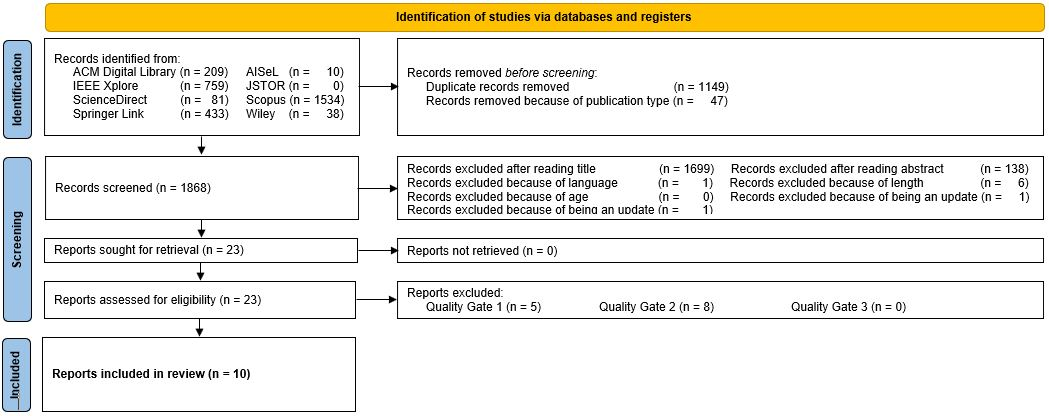
\includegraphics[width=14cm]{Media/PRISMA-Flowchart-Compact.JPG}
        \caption{Overview of the search process}
        \label{fig:PRISMA}
    \end{figure}
    
    % \subsection{Evaluating papers based on inclusion and exclusion criteria}
    
    The remaining 1868 papers were filtered by title to evaluate their relevance to the concepts of microservice patterns or architectural constructs related to MS. For this purpose, the first two authors separately evaluated each entry. If both agreed, this verdict was honored. In case of disagreement, they discussed the title to come to a conclusion. In this phase 1699 papers were excluded. The same approach was followed for abstracts. next, out of 169 remaining papers, 138 papers has been exluceded. From there on, the papers that were not written in English (despite the abstract being in English), were published before the year 2012, and had a length of less than six pages were removed. 23 papers have been selected for the quality assement against the quality framework. The agreement rate among researchers for this phase equates to 88 percent. 
    
    % the first author initially included 113 papers and the second author 146. Of those, 41 were present in both sets and 1650 were excluded by both. 
    
    % This equates to an agreement rate of 90,5 percent (1691 of 1868 records) between the authors. After discussing the contributions with divergent evaluations, in total, 1699 of the 1868 papers were excluded, leaving 169 items for the next round. 
    
    %  As a result, the first author evaluated 40 papers positively, and the second one 28. Both agreed on the inclusion of 22 papers and the exclusion of 123. This equates to an agreement rate of 85,8 percent (145 of 169 records) between the authors. In total of the 169 papers, 138 were removed and 31 were included in the next phase. From there on, the papers that were not written in English (despite the abstract being in English), were published before the year 2012, and had a length of less than six pages were removed.
    
    % It was stipulated so if the agreement could not be reached, an arbitrator would be invited to the research Yet, this was not necessary. 
    
    
    
    % With a difference that authors agreed to also allow themselves to look into the actual paper and not just the abstract, if they wanted to further explore certain aspects of the study to improve their judgement.
    
    
    
    % While conducting the first steps of our filter process, we encountered several hurdles that shall be highlighted to ensure transparency, especially since they can slightly affect the number of remaining entries after those initial phases. However, the final set of literature was not impacted and, therefore, those factors did not pose a threat to the studies validity. For once, since not all entries of the combined literature list specified a digital object identifier (DOI), the duplicate removal had to be conducted based on the publication title. Yet, in some rare cases, there were duplicates for which the spelling of the title was slightly altered (e.g., the two parts of a title were in one search engine separated by a hyphen and in another by a double colon), and which were, therefore, not detected in the initial duplicate removal phase. Instead, they were only identified during the scanning of the title. 
    
    % Furthermore, in SpringerLink, conference papers are classified as book chapter, since conference proceedings are published as books. This makes them indistinguishable from real book chapters, when only looking at the metadata. Book chapters are, however, not part of the search’s scope. Consequently, the removal of book chapters for SpringerLink could only be processed when inspecting the respective publications. To slightly reduce the effort, it was decided to only do this for those publications that passed the filtering by title.
    
    
    
    % However, while there were three corresponding records in the initially obtained set of literature (from the years 2003, 2007, and 2010), those were already filtered out for other reasons by this stage. 
    
    
    % \subsection{Evaluating papers based on the quality framework}
    
    % After having filtered out the pooled studies based on inclusion and exclusion criteria, we initiated a deeper probing, by running the remaining studies against the quality framework. 
    
    
    
    %  For this purpose, studies were evaluated for their content to see if they are actual research or just a mere report on some lessons or expert opinions. In addition, we checked if objectives, justification, aim and context of the studies are clearly communicated.
    
    % This last criterion is primarily geared towards actual experiments. In the conducted literature search, primarily literature-based studies were found, which somewhat devalues this aspect. Nevertheless, to assure completeness, it was still evaluated. 
    
    
    In the first phase, the aim was to ensure that reports fulfill at least a desired minimum level of comprehensiveness. Authors independently rated the three aspects for all 23 remaining papers, giving one point respectively, if they deemed a criterion fulfilled and no point if they considered that aspect lacking. For passing the first phase at least 5/6 points required. In this phase 5 papers have been exlcuded. In the second phase, studies were judged based on their research design and the data collection methods. Minimum rating to pass was 3/4 and 8 papers has been excluded. Finally, the remaining 10 papers went through the third. Here, the credibility of the reporting and the relevance of the findings were evaluated. No paper has been removed in this phase.
    
    The overall agreement rate between researchers is 71.6 percent. All ten studies selected have been published in 2018 or later, with three of them being published in 2022, which shows the timeliness of the topic. Eight of the ten papers were found via Scopus, whereas the remaining two have been identified through IEEE Xplore. These papers are described in \citet{foundPapers}.

    \item[Data Synthesis:] After selecting the quality papers, we embarked on the data synthesis process. For this phase we follow the guidelines of thematic synthesis discussed by Cruzes et al. \citet{Cruzes.2011}. To begin, we first extracted the following data from each paper: 1) findings, 2) research motivation, 3) author, 4) title, 5) research objectives, 6) research method, 7) year. We extracted these data through coding, using the software Nvivo. After that, we created two codes: 1) patterns, and 2) BD requirements, and coded the findings based on it. By the end of this process, various themes emerged. 
    
\end{description}

% \subsection{}



% These search terms are chosen because \emph{patterns} are exactly what was sought for, \emph{architectures} can contain such patterns, and \emph{design} is often used as a synonym for architecture. Further, patterns can be seen as \emph{building blocks}, therefore, the building blocks was also included. 

% Finally, the use of patterns is often highlighted as a best practice and hence, in reverse, papers that refer to best practices might also contain information regarding the use of patterns. 


% For those engines that yielded a high number of results, the scope was reduced by adding variations of “pattern”, “architecture”, “design”, “building block”, or “best practice” to appear in title, abstract or keywords.

% Table \ref{table:searchTerms} depicts the resulting mapping of databases and search terms. 

% If a term in the “Search Term” column is printed in bold, this indicates a field of the search mask, where the following text is input. In case nothing is printed in bold, this means the whole term can be filled into the search bar without modification. As can be seen, due to the focus of this study, the term “microservice” or its plural always had to be included in the title.

%  If this could not be realized because of the interface, the most similar setting that is more lenient (therefore, potentially yielding more results) was chosen. This was the case for IEEE Xplore and SpringerLink. 
 



% \begin{table*}[h]
%     \renewcommand{\arraystretch}{1.5}
%     \caption[]{Mapping of databases/registers and search terms}
%     \begin{tabular}{|p{5cm}|p{10cm}|p{2cm}|}
%         \hline
%         Database/Register & Search Term & Records \\ 

%         \hline
%         ACM Digital Library (“The ACM Full-Text Collection”, not “The ACM Guide to Computing Literature
%         &  
        
        
%         1) [Title: microservice*] AND [[Title: pattern*] OR [Title: architecture*] OR [Title: design*] OR [Title: building block*] OR [Title: best practice*]]
        
%         \hspace{1cm}

%         2) [Title: microservice*] AND [[Abstract: pattern*] OR [Abstract: architecture*] OR [Abstract: design*] OR [Abstract: building block*] OR [Abstract: best practice*]]

%         \hspace{1cm}

%         3) [Title: microservice*] AND [[Keywords: pattern*] OR [Keywords: architecture*] OR [Keywords: design*] OR [Keywords: building block*] OR [Keywords: best practice*]]
%         & 
%         1) 91



%         2) 194



%         3) 65
        
%         \\ 

%         \hline
%         AISeL & \textbf{Title}: microservice OR microservices & 10 \\ 
%         \hline

%         IEEE Xplore & "Document Title": microservice*  AND ("All Metadata": pattern* OR "All Metadata": architecture* OR "All Metadata": design* OR "All Metadata": building block* OR "All Metadata": best practice*)  & 759 \\ 
%         \hline

%         JSTOR & 
        
%         \textbf{Title:} microservice 

%         \textbf{Title:} microservices 
%         & 0 \\ 

%         \hline

%         ScienceDirect & 
        
%         1) \textbf{Title, abstract, keywords}: pattern OR architecture OR design OR (building block) OR (best practice)

%            \textbf{Title}: microservice OR microservices

%         2) \textbf{Title, abstract, keywords}: patterns OR architectures OR designs OR (building blocks) OR (best practices)

%             \textbf{Title}: microservice OR microservices
%         & 
%         1) 79

%         2) 76
%         \\ 

%         \hline

%         Scopus & ( TITLE-ABS-KEY ( pattern*  OR  architecture*  OR  design*  OR  ( "building block" )  OR  ( "building blocks" )  OR  ( "best practice" )  OR  ( "best practices" ) )  AND  TITLE ( microservice* ) ) & 1534 \\ 
%         \hline

%         SpringerLink & \textbf{Title}: microservice*


%         \textbf{With at least one of the words}: pattern* architecture* design* "building block" "building blocks" "best practice" "best practices
%          & 433 \\ 
%         \hline

%         Wiley & \textbf{Title}: microservice* & 38 \\ 

%         \hline
%     \end{tabular}
    
%     \label{searchTerms}
% \end{table*}

% As it can be seen at \citet{SLRsearchTerms}, due to the specifics of their search masks, the searches in the ACM Digital Library (title, abstract, keywords could only be searched separately), JSTOR (no support of wildcards), and Science Direct (no support of wildcards) had to be split in several parts. Those were afterwards merged for each of them, and duplicates were removed. 

% \subsection{Developing inclusion, exclusion criteria and the quality framework}

% Inspired by PRISMA checklist presented by \citet{tricco2018prisma}, Our inclusion and exclusion criteria are formulated as following:

% \textbf{Inclusion Criteria:} 1) Primary and secondary studies between Jan 1st 2012 and June 19th 2022, 2) The focus of the study is on MS patterns, and MS architectural constructs, 3) Scholarly publications such as conference proceedings and journal papers.

% \textbf{Exclusion Criteria:} 1) Studies that are not written in English, 2) Informal literature surveys without any clearly defined research questions or research process, 3) Duplicate reports of the same study (a conference and journal version of the same paper). In such cases, the conference paper was removed. 4) Complete duplicates (not just Updates) were also removed. 5) Short papers (less than 6 pages).

% % \subsection{Developing the quality framework}
% \textbf{Quality Framework:} Quality of the evidence collected as a result of this SLR has direct impact on the quality of the findings, making quality assessment an important undertaking. To address this, we developed a criteria made up of 7 elements. These criteria are informed by guidelines provided by Kitchenham \citet{Kitchenham.2004} on empirical research in software engineering. These 7 criteria are applied in three different stages (quality gates). These 7 criteria are discussed in Table \ref{qualityFramework}.


% \begin{enumerate}
%     \item 
%     \item The focus of the study is on microservices patterns, and microsrvices architectural constructs.
%     \item Scholarly publications such as conference proceedings and journal papers
% \end{enumerate}

% \subsection{Pooling literature based on the search strategy}
% \subsection{Pooling literature and evaluation}

% Overall, the keyword search yielded 3064 contributions. The total number of found publications per source as well as an overview of the further search process can be seen in Figure 1.

% \begin{figure}
%     \centering 
%     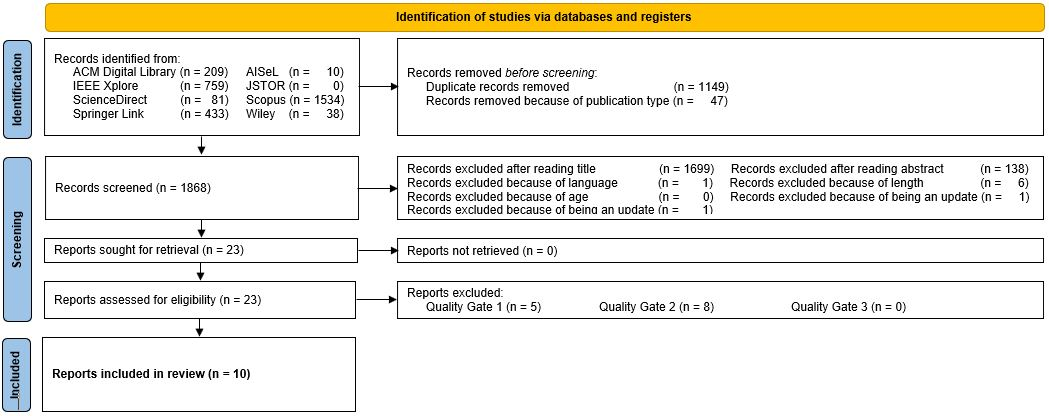
\includegraphics[width=14cm]{Media/PRISMA-Flowchart-Compact.JPG}
%     \caption{Overview of the search process}
%     \label{fig:PRISMA}
% \end{figure}

% \subsection{Evaluating papers based on inclusion and exclusion criteria}

% The remaining 1868 papers were filtered by title to evaluate their relevance to the concepts of microservice patterns or architectural constructs related to MS. For this purpose, the first two authors separately evaluated each entry. If both agreed, this verdict was honored. In case of disagreement, they discussed the title to come to a conclusion. In this phase 1699 papers were excluded. The same approach was followed for abstracts. next, out of 169 remaining papers, 138 papers has been exluceded. From there on, the papers that were not written in English (despite the abstract being in English), were published before the year 2012, and had a length of less than six pages were removed. 23 papers have been selected for the quality assement against the quality framework. The agreement rate among researchers for this phase equates to 88 percent. 

% the first author initially included 113 papers and the second author 146. Of those, 41 were present in both sets and 1650 were excluded by both. 

% This equates to an agreement rate of 90,5 percent (1691 of 1868 records) between the authors. After discussing the contributions with divergent evaluations, in total, 1699 of the 1868 papers were excluded, leaving 169 items for the next round. 

%  As a result, the first author evaluated 40 papers positively, and the second one 28. Both agreed on the inclusion of 22 papers and the exclusion of 123. This equates to an agreement rate of 85,8 percent (145 of 169 records) between the authors. In total of the 169 papers, 138 were removed and 31 were included in the next phase. From there on, the papers that were not written in English (despite the abstract being in English), were published before the year 2012, and had a length of less than six pages were removed.

% It was stipulated so if the agreement could not be reached, an arbitrator would be invited to the research Yet, this was not necessary. 



% With a difference that authors agreed to also allow themselves to look into the actual paper and not just the abstract, if they wanted to further explore certain aspects of the study to improve their judgement.



% While conducting the first steps of our filter process, we encountered several hurdles that shall be highlighted to ensure transparency, especially since they can slightly affect the number of remaining entries after those initial phases. However, the final set of literature was not impacted and, therefore, those factors did not pose a threat to the studies validity. For once, since not all entries of the combined literature list specified a digital object identifier (DOI), the duplicate removal had to be conducted based on the publication title. Yet, in some rare cases, there were duplicates for which the spelling of the title was slightly altered (e.g., the two parts of a title were in one search engine separated by a hyphen and in another by a double colon), and which were, therefore, not detected in the initial duplicate removal phase. Instead, they were only identified during the scanning of the title. 

% Furthermore, in SpringerLink, conference papers are classified as book chapter, since conference proceedings are published as books. This makes them indistinguishable from real book chapters, when only looking at the metadata. Book chapters are, however, not part of the search’s scope. Consequently, the removal of book chapters for SpringerLink could only be processed when inspecting the respective publications. To slightly reduce the effort, it was decided to only do this for those publications that passed the filtering by title.



% However, while there were three corresponding records in the initially obtained set of literature (from the years 2003, 2007, and 2010), those were already filtered out for other reasons by this stage. 


% \subsection{Evaluating papers based on the quality framework}

% After having filtered out the pooled studies based on inclusion and exclusion criteria, we initiated a deeper probing, by running the remaining studies against the quality framework. 



%  For this purpose, studies were evaluated for their content to see if they are actual research or just a mere report on some lessons or expert opinions. In addition, we checked if objectives, justification, aim and context of the studies are clearly communicated.

% This last criterion is primarily geared towards actual experiments. In the conducted literature search, primarily literature-based studies were found, which somewhat devalues this aspect. Nevertheless, to assure completeness, it was still evaluated. 


% In the first phase, the aim was to ensure that reports fulfill at least a desired minimum level of comprehensiveness. Authors independently rated the three aspects for all 23 remaining papers, giving one point respectively, if they deemed a criterion fulfilled and no point if they considered that aspect lacking. For passing the first phase at least 5/6 points required. In this phase 5 papers have been exlcuded. In the second phase, studies were judged based on their research design and the data collection methods. Minimum rating to pass was 3/4 and 8 papers has been excluded. Finally, the remaining 10 papers went through the third. Here, the credibility of the reporting and the relevance of the findings were evaluated. No paper has been removed in this phase.

% The overall agreement rate between researchers is 71.6 percent. All ten studies selected have been published in 2018 or later, with three of them being published in 2022, which shows the timeliness of the topic. Eight of the ten papers were found via Scopus, whereas the remaining two have been identified through IEEE Xplore. These papers are described in \citet{foundPapers}.




% Authors independently rated the three aspects for all 23 remaining papers, giving one point respectively, if they deemed a criterion fulfilled and no point if they considered that aspect lacking. For inclusion into the second phase, at least five out of six points were demanded to assure a sufficient base quality. This corresponds to having at least 75 percent of the points. In total, the authors agreed on 51 of 69 evaluations, resulting in an agreement rate of 73,9 percent. The second phase was focused on rigor. 

% Two papers that obtained four out of six points were again discussed between the two authors to avoid any erroneous exclusion.

% Despite that additional check, both were still removed. 

% The second phase was focused on rigor. In this phase, studies were judged based on their research design and the data collection methods. For inclusion in the next phase, again, 75 percent of the obtainable point were needed (this time three out of four). In total, the authors agreed on 23 of 36 evaluations, resulting in an agreement rate of 63,9 percent. The papers with the highest score (this time two) were discussed before inclusion, to further counteract possible fuzziness in the individual evaluations.  

% While this value is rather low, this is likely caused by the narrow margins for some decisions. 



% The remaining 10 papers went through the third and final phase. Here, the credibility of the reporting and the relevance of the findings were evaluated. In this last phase, the authors agreed on 14 of 20 evaluations, resulting in an agreement rate of exactly 70 percent. All ten publications have been published in 2018 or later, with three of them being published in 2022, which shows the timeliness of the topic. Eight of the ten papers were found via Scopus, whereas the remaining two have been identified through IEEE Xplore. These papers are described in \citet{foundPapers}.


% \subsection{Data synthesis}

% After selecting the quality papers, we embarked on the data synthesis process. For this phase we follow the guidelines of thematic synthesis discussed by Cruzes et al. \citet{Cruzes.2011}. To begin, we first extracted the following data from each paper: 1) findings, 2) research motivation, 3) author, 4) title, 5) research objectives, 6) research method, 7) year. We extracted these data through coding, using the software Nvivo. After that, we created two codes: 1) patterns, and 2) BD requirements, and coded the findings based on it. By the end of this process, various themes emerged. 



% Consequently, for the search conducted for this paper, the other databases and registers have not been necessary. However, since this fact is only determinable now, their inclusion in the initial search was still sensible.

% Pouya


\section{Second Review}

The second SLR is conducted by \citet{ataei2022state} on available BD RAs in academia and industry. This is comprehensive study that covers various aspects of BD RAs such as limitations, and common architectural blocks. The findings from this SLR helped us shaped the requirements necessary for BD systems. We do not explore this SLR in this paper, and aim to only discuss the results of it.


% While the common architectural constructs was discussed in in this study, the focus was not on BD system requirements. 


% Therefore, we assessed and coded the findings of this SLR to point out the system requirements of BD systems. This was achieved by creating a new code in Nvivo called: 'software and system requirements'. This was necessary as we needed to map patterns against requirements. This is further elaborated in the results section. Requirements were further explored from other studies which is discussed in Section~\ref{requirements}


\chapter{Results}


In this section, we present with three integral elements: 1) BD software and system requirements, 2) MS patterns, 3) the mapping between the two and theories that emerged as a result.  

\section{Big Data Software and System Requirements}\label{requirements}

While we could find BD major building blocks and system requirements by coding the findings gained from \citet{ataei2022state} work, our coding process did not include categorization and representation of these requirements. To this end, we performed a lightweight literature review in the body of knowledge to realize what type of requirement is needed, how these requirements are categorised and what's the best way to present them. The results are as following:

\begin{enumerate}
    \item \textbf{Type of requirements:} For the purposes of this study, we opted for a well-received approach discussed by \citet{laplante2017requirements}. In this approach, requirements are classified into three major types of 1) functional requirements, 2) non-functional requirements, and 3) domain requirements. Our primary focus is one functional and domain requirements. 
    \item \textbf{Categorizing Requirements:} For categorization of requirements, we followed the well-established categorization method based on BD characteristic, that is the 5Vs. These 5Vs are velocity, veracity, volume, variety and value \citep{rad2017big}. We took inspiration from various studies such as the work of \citet{nadal2017software}, and the requirements categories presented in NIST BD Public Working Group \citep{Chang.2019}. This resulted in addition of `security and privacy' to the category of requirements. We do not aim to define these characteristics in this study. This can be found in the works of \citet{rada2017hype}.
    \item \textbf{Presenting Requirements:} For the purposes of this study, we opted for an informal method because it is a well established method in the industry and academia \citep{kassab2014state}. Our approach follows the guidelines explained in ISO/IEC/IEEE standard \citet{ISO29148} for representing functional requirements. These requirements are described in Table \ref{table-requirements}.
    \begin{table*}[h]
        \centering
        \caption{BD system requirements}
        \renewcommand*{\arraystretch}{1.1}
        \begin{tabular}{|m{1.2cm}|m{14cm}|}
    
            \hline
    
            Volume &
    
            \textbf{Vol-1)} System needs to support asynchronous, streaming, and batch processing to collect data from centralized, distributed, and other sources, \textbf{Vol-2)} System needs to provide a scalable storage for massive data sets 
            \\
            \hline
            Velocity & 
            
            \textbf{Vel-1)} System needs to support slow, bursty, and high-throughput data transmission between data sources, \textbf{Vel-2)} System needs to stream data to data consumers in a timely manner, \textbf{Vel-3)} System needs to be able to ingest multiple, continuous, time varying data streams, \textbf{Vel-4)} System should be able to process data in real-time or near real-time manner 
            \\ 
    
            \hline
    
            Variety & 
    
            \textbf{Var-1)} System needs to support data in various formats ranging from structured to semi-structured and unstructured data, \textbf{Var-2)} System needs to support aggregation, standardization, and normalization of data from disparate sources, \textbf{Var-3)} System shall support adaptations mechanisms for schema evolution, \textbf{Var-4)} System can provide mechanisms to automatically include new data sources 
            \\
    
            \hline
    
            Value & 
            
            \textbf{Val-1)} System needs to able to handle compute-intensive analytical processing and machine learning techniques, \textbf{Val-2)} System needs to support two types of analytical processing: batch and streaming, \textbf{Val-3)} System needs to support different output file formats for different purposes, \textbf{Val-4)} System needs to support streaming results to the consumers 
            \\
    
            \hline
    
            Security \& Privacy & 
            
            \textbf{SaP-1)} System needs to protect and retain privacy and security of sensitive data, \textbf{SaP-2)} System needs to have access control, and multi-level, policy-driven authentication on protected data and processing nodes. 
            \\
    
            \hline
            
            Veracity &
            
            \textbf{Ver-1)} System needs to support data quality curation including classification, pre-processing, format, reduction, and  transformation, \textbf{Ver-2)} System needs to support data provenance including data life cycle management and long-term preservation.
            \\
            \hline
      
        \end{tabular}
        \label{table-requirements}
        \end{table*}

\end{enumerate}


% \subsection{Type of requirements}
% System and software requirements come in different flavours and can range from a formal (mathematical) specifications to sketch on a napkin. There's been various attempts to defining and classifying software and system requirements. For the purposes of this study, we opted for a well-received approach discussed by \citet{laplante2017requirements}. In this approach, requirements are classified into three major types of 1) functional requirements, 2) non-functional requirements, and 3) domain requirements. 

% Our objective is to define the high-level requirements of BD systems, thus we do not fully explore 'non-functional' requirements. Majority of non-functional requirements are emerged from the particularities of an environment, such as a banking sector or healthcare, and do not correlate to our study. Our primary focus is one functional and domain requirements. 

% \subsection{Categorizing requirements} After having filtered out the right type of requirement, we then sought for a rigorous and relevant method to categorize the requirements. For this purpose, we followed the well-established categorization method based on BD characteristics, that is the 5Vs. These 5Vs are velocity, veracity, volume, variety and value \citep{Bughin2016,rad2017big}. We took inspiration from various studies such as the work of \citet{nadal2017software}, and the requirements categories presented in NIST BD Public Working Group \citep{Chang.2019}.

% have underpinned their reference architecture on these characteristics and requirements that goes with them. Moreover, NIST BD Public Working Group embarked on a large scale study to extract requirements from variety of application domains such as Healthcare, Life Sciences, Commercial, Energy, Government, and Defense. The result of this study was the formation of general requirements under seven categories. In another effort by Volk et al. (\citet{volk2020identifying}), nine use cases for BD projects are identified by collecting theories and use cases from the literature and categorizing them using a hierarchical clustering algorithm. 

% Bashari et al. (\citet{bashari2016security}) focused on the security and privacy requirements of BD systems, Yu et al. presented the modern components of BD systems (\citet{yu2019components}), Eridaputra et al. (\citet{eridaputra2014modeling}) created a generic model for BD requirements using goal oriented approaches, and Al-jaroodi et al. (\citet{al2016characteristics}) investigated general requirements to support BD software development. 

% In addition, we studied the RAs developed for BD systems to understand general requirements. For this purpose, we used the SLR published by \citet{ataei2022state}. This SLR assessed the body of evidence and presented with a comprehensive list of BD RAs. This study helped us realize the spectrum of BD RAs, how they are designed and the general set of requirements. By evaluating the design and requirement engineering required for BD RAs, we adjusted our initial categories of requirements and added security and privacy to it. 

% \subsection{Present requirements}
% After knowing the type and category of requirements, We looked for a rigorous approach to present these requirements. There are numerous approaches used for software and system requirement representation including informal, semiformal and formal methods. For the purposes of this study, we opted for an informal method because it is a well established method in the industry and academia \citep{kassab2014state}. Our approach follows the guidelines explained in ISO/IEC/IEEE standard \citet{ISO29148} for representing functional requirements. We have also taken inspiration from Software Engineering Body of Knowledge \citep{abran2004software}. However, our requirement representation is organized in term of BD characteristics. These requirements are described in Table \ref{table-requirements}.





\section{Microservice Patterns}

As a result of this SLR, our data synthesis yielded 50 MS patterns. These patterns are classified based on their function and the problem they solve. While we elaborate the patterns adopted for BD requirements in detail, the aim of our study is not to explain each MS pattern. Nevertheless, the name of all patterns found and their category can be found in \citet{MSPatterns}. Additionally the definition of these patterns with examples can be found in the works of \citet{richardson2018microservices}.

  
% \begin{center}
%     \begin{table*}
%     \renewcommand*{\arraystretch}{1.8}
%     \begin{tabular}{ | m{3cm} | m{12cm} | }

%         \hline

%         Category & Pattern
 
%         \\

%         \hline

%         Data Management &  Database per Service, Shared Database, Event Sourcing, Command and Query Responsibility Segregation
 
%         \\

%         \hline

%         Platform and Infrastructure & Multiple service instances per host, External configuration store, Sidecar, Static content hosting, Computer resource consolidation
 
%         \\

%         \hline

%         Communicational & API gateway,  Anti-corruption layer, Self Registration, Service Discovery, Competing consumers, Pipes and filters, Priority queue, Ambassador, Gateway aggregate, Gateway offloading, Aggregator, Backend for Frontend, API Composition, Saga transaction management, Gateway routing, Leader election
        
 
%         \\

%         \hline

%         Fault Tolerance & Circuit breaker, Bulkhead pattern
 
%         \\
%         \hline

%         Observability & Log Aggregation Pattern
 
%         \\
%         \hline


%     \end{tabular}
%     \caption{Microservices categorization}
%     \label{microservices-categorization}
%     \end{table*}
% \end{center}


% \begin{center}
%     \begin{table*}
%     \renewcommand*{\arraystretch}{1.8}
%     \begin{tabular}{ | m{2cm} | m{8cm} |  m{2cm} |}

%         \hline

%         Requirement &  Patterns & Reasoning
 
%         \\
%         \hline

%         Vol-1 &  
        
%         1) Database per Service

%         2)  Event Sourcing
        
%         3)  Command and Query Responsibility Segregation
        
%         4)  External Configuration Store
        
%         5)  API gateway
        
%         6)  Anti-Corruption Layer
        
%         7)  Service Discovery
        
%         8)  Self Registration
        
%         9)  Priority Queue

%         10) Gateway Offloading 

%         11) Gateway Aggregate 

%         12) Leader Election

%         13) Log Aggregation Pattern 
        
%         & Reasoning 
 
%         \\

%         \hline

%         Vol-2 &  
        
%         1) Database per Service  
        
%         2) Command and Query Responsibility Segregation
        
%         & Reasoning
        
%         \\
%         \hline

%         Vel-1 &  
    
%         1) API Gateway 

%         2) Service Discovery 

%         3) Pipes and Filters 

%         4) Leader Election 

%         5) Circuit Breaker 

%         6) Log Aggregation  
        
%         & Reasoning
        
%         \\
%         \hline

%         Vel-2 &  
    
%         1) Command and Query Responsibility Segregation
        
%         2) API gateway

%         3) Competing consumers

%         4) Gateway aggregate

%         5) Gateway Offloading

%         6) Leader Election 

%         & Reasoning

%         \\

%         \hline

%         Vel-3 &  
    
%         1) Command and Query Responsibility Segregation
        
%         2) API gateway

%         3) Competing consumers

%         4) Gateway aggregate

%         5) Gateway Offloading

%         6) Leader Election 

%         & Reasoning
        
%         \\
%         \hline

%         \hline

%         Vel-3 &  

%         1) API composition
        
%         2) API gateway

%         4) Gateway aggregate

%         5) Gateway Offloading

%         & Reasoning
        
%         \\
%         \hline

%         Vel-4 &  

%         1) API composition
        
%         2) API gateway

%         4) Gateway aggregate

%         5) Gateway Offloading
                
%         6) Event Sourcing

%         7) Command and Query Responsibility Segregation

%         & Reasoning
        
%         \\
%         \hline

%         Vel-5 &  

%         1) Leader Election 

%         2) Log Aggregation Pattern 

%         & Reasoning
        
%         \\
%         \hline

        
%         Var-1 &  
        
%         None

%         & Reasoning
        
%         \\
%         \hline

%         Var-2 &  
        
%         1)  Database per Service

%         2) API Gateway

%         & Reasoning
        
%         \\
%         \hline

%         Var-3 & None  & Reasoning
        
%         \\
%         \hline

%         Var-4 &  

%         1) API Gateway

%         2) Gateway Offloading

%         3) Gateway Aggregate
        
%         & Reasoning
        
%         \\
%         \hline
  
%     \end{tabular}
%     \end{table*}
% \end{center}


% \begin{center}
%     \begin{table*}
%     \renewcommand*{\arraystretch}{1.8}
%     \begin{tabular}{ | m{2cm} | m{8cm} |  m{2cm} |}
%         \hline

%         Val-1 &  

%         1) Event Sourcing

%         2) Command and Query Responsibility Segregation

%         3) Priority Queue

%         4) Leader Election

%         5) Bulkhead Pattern
        
%         &  Reasoning 
        
%         \\
%         \hline

%         Val-2 &  

%         1) Event Sourcing

%         2) Command and Query Responsibility Segregation

%         3) API gateway, Gateway aggregate

%         4) Gateway offloading

%         5) Priority queue
        
%         & Reasoning
        
%         \\
%         \hline

%         Val-3 &  

%         1) API gateway

%         2) Anti-corruption layer

%         3) Service Discovery

%         4) Gateway aggregate

%         5) Backend for Frontend
        
%         & Reasoning
        
%         \\
%         \hline

%         Val-4 &  

%         1) Event Sourcing

%         2) Command and Query Responsibility Segregation

%         3) Backend for Frontend

%         & Reasoning
        
%         \\
%         \hline

%         SaP-1 &  

%         1) External Configuration Store

%         2) API Gateway

%         3) Gateway Aggregate

%         4) Backend for Frontend 
        
%         & Reasoning
        
%         \\
%         \hline

%         SaP-2 &  

%         1) External Configuration Store

%         2) API Gateway

%         3) Gateway Aggregate

%         4) Backend for Frontend 
        
%         & Reasoning
        
%         \\
%         \hline

%         Ver-1 &  

%         1) Pipes and filters
        
%         & Reasoning
        
%         \\
%         \hline

%         Ver-2 &  
%         None 
%         & Reasoning
        
%         \\
%         \hline

        
%         Ver-3 &  
        
%         None

%         & Reasoning
        
%         \\
%         \hline

             
%         Ver-4 &  
        
%         1) Circuit Breaker

%         & Reasoning
        
%         \\
%         \hline

%     \end{tabular}
%     \end{table*}
% \end{center}


\chapter{Application of Microservices Design Patterns to Big Data Systems}


In this section, we combine our findings from both SLRs, and present new theories on application of MS design patterns for BD systems. The patterns gleaned are established theories that are derived from actual problems in MS systems in practice, thus we do not aim to re-validate them in this study. The main contribution of our work is to propose new theories in regards to application of MS patterns to BD systems. To achieve this, we map BD system requirements against a pattern and provide with reasoning on why such pattern might work for BD systems. We support our arguments by the means of modeling. We use Archimate as our architectural description language. This is recommend in ISO/IEC/IEEE 42010 \citep{Chaabane}. 

% BD systems and microservices architecture are both inherently distributed. While many of the current BD systems are designed underlying a monolithic data pipeline architecture, here, we propose microservices architecture for a domain-driven and decentralized BD architecture.

We posit that a pattern alone would not be significantly useful to a data engineering or a data architect, and propose that a collection of patterns in relation to current defacto standard of BD architectures is a better means of communication. To achieve this, we provide theories on how MS patterns can address BD requirements. Additionally, we portray selected patterns in a reference architecture.


\section{Volume} \label{volumeSection}

% There has been two requirements associated to the Volume aspect of big data systems which are about handling various data types (Vol-1) and providing with a scalable storage (Vol-2). 

To address the volume requirements of BD , and in specific for Vol-1 and Vol-2 we suggest the following patterns to be effective; 1) Gateway offloading, 2) API gateway, 3) External Configuration Store

\vspace{6px}
\textbf{1.Gateway Offloading and API Gateway:} In a typical flow of data engineering, data goes from ingestion, to storage, to transformation and finally to serving. However there are various challenges to maintain this. One challenge is the realization of various data sources as described in Vol-1. Data comes in various formats from and system needs to handle different data through different interfaces. 

% So some of the key engineering consideration for the ingestion process is that; 1) is the BD system ingesting data reliably? How frequently should data be ingested? In what volume the data typically arrives?

Given the challenges and particularities of data types, different nodes may be spawned to handle the volume of data. This can be problematic as different nodes will need to account for cross-cutting concerns such as certificate management, throttling, logging, monitoring and authentication. If each node reimplement the same interface for the cross-cutting concerns, scalability and maintainability can be a daunting task. This also introduces unnecessary repetition of codes and can result in incompatible interfaces. To solve this problem, we explore the concept of gateway offloading. Offloading cross-cutting concerns to a single architectural construct, achieves `separation of concerns'. This simplifies development and removes the need for a re-implementing cross-cutting concerns. In addition, it introduces consistency in terms of logging and monitoring and allow teams to work on things that they are specialized in.

% Another popular approach is the segregation of concerns by separating batch and streaming processing nodes. Given the requirement of horizontal scaling for BD systems, it is safe to assume that there is usually more then one node associated to ingesting data.


Moreover, if data producers directly communicate with the processing nodes, they will have to update the endpoint address every now and on. This issue is exacerbated when the data producer tries to communicate to a service that is down. Given that lifecycle of a service in a typical distributed cloud environment is not deterministic and many container orchestration systems constantly recycle services to proactively address this issue, reliability and maintainability of the BD system can be compromised. This also increases round-trips, and introduces security issues. To address this, we introduce the API gateway pattern. API gateway can be the single point of entry to the system, providing with request aggregation, gateway routing and proxying. This is an effective pattern in tackling cross-cutting concerns specially in distributed system with many nodes. These pattern are portrayed in Figure \ref{fig:RA}. 



% \subsection{Gateway Offloading and API Gateway:} In a typical flow of data engineering, data goes from ingestion, to storage, to transformation and finally to serving. However there are various challenges to maintain this. One challenge is the realization of various data sources as described in Vol-1. Data comes in various formats from and system needs to handle different data through different interfaces. 

% % So some of the key engineering consideration for the ingestion process is that; 1) is the BD system ingesting data reliably? How frequently should data be ingested? In what volume the data typically arrives?

% Given the challenges and particularities of data types, different nodes may be spawned to handle the volume of data. This can be problematic as different nodes will need to account for cross-cutting concerns such as certificate management, throttling, logging, monitoring and authentication. If each node reimplement the same interface for the cross-cutting concerns, scalability and maintainability can be a daunting task. This also introduces unnecessary repetition of codes and can result in incompatible interfaces. To solve this problem, we explore the concept of gateway offloading. Offloading cross-cutting concerns to a single architectural construct, achieves `separation of concerns'. This simplifies development and removes the need for a re-implementing cross-cutting concerns. In addition, it introduces consistency in terms of logging and monitoring and allow teams to work on things that they are specialized in.

% % Another popular approach is the segregation of concerns by separating batch and streaming processing nodes. Given the requirement of horizontal scaling for BD systems, it is safe to assume that there is usually more then one node associated to ingesting data.


% Moreover, if data producers directly communicate with the processing nodes, they will have to update the endpoint address every now and on. This issue is exacerbated when the data producer tries to communicate to a service that is down. Given that lifecycle of a service in a typical distributed cloud environment is not deterministic and many container orchestration systems constantly recycle services to proactively address this issue, reliability and maintainability of the BD system can be compromised. This also increases round-trips, and introduces security issues. To address this, we introduce the API gateway pattern. API gateway can be the single point of entry to the system, providing with request aggregation, gateway routing and proxying. This is an effective pattern in tackling cross-cutting concerns specially in distributed system with many nodes. These pattern are portrayed in Figure \ref{fig:RA}. 

% % on the fence!
% % Additionally, the gateway can increase the system reliability and availability by doing a constant health check on services, and distribute traffic based on liveliness probes. There are other benefits to to these patterns suich as weighted distribution, customized cache mechanism through specific HTTP headers, and consolidated security. This also means that if the gateway is down, service nodes won't introduce bad state into the overall system. We have portrayed a simplistic representation of this pattern in Figure \ref{fig:RA}. 

\vspace{6px}
\textbf{2. External Configuration Store:} As discussed earlier, BD systems are made up of various services in order to achieve horizontal scalability. These services will have to communicate with each other in order to achieve the goal of the system. Thus, each one of them will require a set of runtime environmental configurations. These configurations could be database network locations, feature flags, and third party credentials. Moreover, different stages of the data engineering may have different environments for different purposes, for instance, privacy engineers may require a completely different environment to achieve their requirements. 

Therefore, the challenge is the management of these configurations as the system scales, and enabling services to run in different environments without modification. To address this problem, we propose the external configuration store pattern. By externalizing all nodes configuration to another service, each node can request its configuration from an external store on boot up. This pattern solves the challenges of handling large number of nodes in BD systems and provide with a scalable solution for handling configurations. This pattern is portrayed in Figure \ref{fig:RA}.

\begin{figure*}[h]
    \centering 
    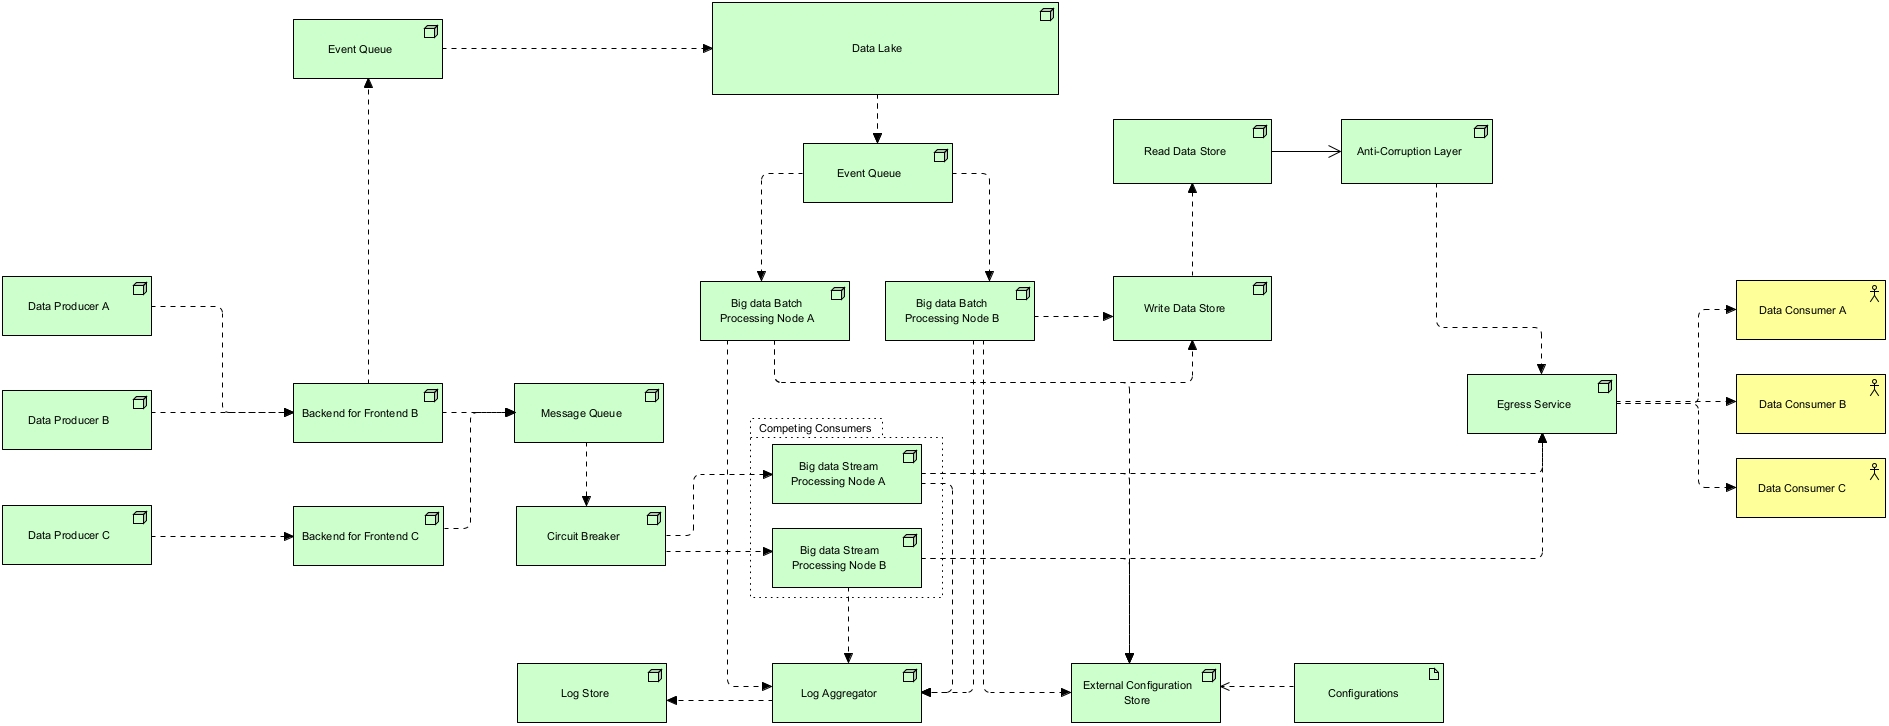
\includegraphics[width=16.5cm]{Media/All together.jpg}
    \caption{Big data reference architecture with microservices patterns}
    \label{fig:RA}
\end{figure*}

\section{Velocity}

To address some of the challenges associated with the velocity aspect of BD systems, we recommend the following patterns for the requirements Vel-1, Vel-2, Vel-3, and Vel-4; 1) Competing Consumers, 2) Circuit Breaker and 3) Log Aggregation.

\vspace{6px}
\textbf{1. Competing Consumers:} According to a recent MIT report in collaboration with Databricks, one of the main challenges of BD 'low-achievers' is the 'slow processing of large amounts of data' \citep{DataBricksSurvey}. If the business desires to go data driven, it should be able to have an acceptable time-to-insight. 

% Given the very contrived scenario of a BD system described in the previous section, at the very core, 

Data needs to be ingested quickly, stored in a timely manner, batch, or stream processed, and served to the consumers. So what happens if one node goes down or becomes unavailable? The system has to wait, the node becomes unavailable, and any workload for stream processing comes to halt, failing to achieve requirements Vel-2, Vel-3 and Vel-4. This issue is exacerbated if the system is designed and architected underlying monolithic pipeline architecture with point-to-point communications. One way to solve some of these issues, is to introduce a non-blocking asynchronous event driven communication style to increase fault tolerance and availability. In this communication style, there's a producer that produces the event, the message queueing system that transfers the message and a consumer that consumes the message. This communication is logically separated in topics. 

While this communication may improve the availability and idle time, it can fail due to sudden increase in the number of requests. This is because the consumer that receives the message may not be unhealthy and unavailable.To address this challenge, we can adopt the competing consumer pattern. Adopting this pattern means instead of one consumer listening on the topic, there will be a few. This means if one node is down, other nodes can listen to the incoming event. In this paradigm, message queue distributes the traffic to healthy consumers and avoid the unhealthy ones. This improves scalability, reliability, and resiliency. This pattern will help alleviate challenges in regards to Vel-2, Vel-3 and Vel-4. This pattern is portrated in Fig \ref{fig:RA}.

% as portrayed in the works of \citet{ataei2021neomycelia}, and try to increase fault tolerance and availability through competing consumers, circuit breaker, and log aggregation. 

% in a traditional Hadoop setup, if Mesos is utilized as the scheduler, the node will be restarted and will go through a lifecycle again. 



% Underlying the event-driven approach, nodes are sending each other events as a means of communication. This implies that node A can send an event to node B in a 'dispatch and forget' model on a certain topic. However this communication style introduces the same problem as the point-to-point communication style. 



% This can change the nature of the communication to asynchronous mode, and allow for a better fault tolerance, because if one node is down, the other nodes can listen to the event and handle it. In other terms, because now there are a few consumers listening on the events being dispatched on a certain topic, there's a competition of consumers, therefore the name 'competing consumers'. 

\vspace{6px}
\textbf{2. Circuit Breaker:} On the other hand, given the large number of nodes one can assume for any BD system, one can employ the circuit breaker pattern to signal the service unavailability. Circuit breakers can protect the overall integrity of data and processes by tripping and closing the incoming request to the unhealthy service. This communicates effectively to the rest of the system that the node is unavailable, allowing engineers to handle such incidents gracefully. This pattern, mixed with competing consumers pattern can increase the overall availability and reliability of the system, and this is achieved by providing an even-driven asynchronous fault tolerance communication mechanisms among BD services. This allows system to be able to be resilient and responsive to bursty, high-throughput data as well as small, batch oriented data, addressing requirements Vel-1, Vel-4, and Vel-4. 
    
\vspace{6px}
\textbf{3. Log Aggregator:} Given that BD systems are comprising of many services, log aggregation can be implemented to shed lights on these services and their audit trail. Traditional single node logging does not work very well in distributed environments, as engineers are required to understand the whole flow of data from one end to another. To address this issue, log aggregation can be implemented, which usually comes with a unified interface that services communicate to and log their processes from. This interface then, does the necessary processes on the logs, and finally store the logs. 

In addition, reliability engineers can configure alerts to be triggered underlying certain metrics. This increases teams agility to proactively resolve issues, which in turn increases reliability and availability which in turn addresses the velocity requirement of BD systems. While this design pattern does not directly affect any system requirements, it indirectly affects all of them. A simplistic presentation of this pattern is portrayed in Figure \ref{fig:RA}. 


% \begin{figure*}[h!]
%     \includegraphics[width=17cm]{../Media/Velocity Requirement.jpg}
%     \caption{Design patterns for velocity requirements}
%     \label{fig-vel-ra}
% \end{figure*}


\section{Variety}
To address some of the challenges of this endeavour, we recommend the following patterns to address requirements Var-1, Var-3, Var-4; 1) API Gateway, 2) Gateway Offloading.

\vspace{6px}
\textbf{1. API Gateway and Gateway Offloading:} We have previously discussed the benefits of API Gateway and Gateway Offloading, however in this section we aim to relate it more to BD system requirements Var-1, Var-3, and Var-4. Data engineers need to keep an open line of communication to data producers on changes that could break the data pipelines and analytics. Suppose that developer A changes a field in a schema of an object that may break a data pipeline or introduce a privacy threat. How can data engineers handle this scenario effectively? 

To address this problem, API Gateway and Gateway Offloading can be used. These patterns can be used to offload some of the light-weight processes that may be associated to the data structure or the type of data. Moreover, as the data engineering loads increases, there will be more servers spawned for batch and stream processing. Gateways help with handling the traffic to these new servers and provide with zero down-time transitions. High-level overview of API Gateway pattern is portrayed in Figure \ref{fig:RA}.

\section{Value}

To address some of these challenges, we propose the following patterns to address the requirements Val-1, Val-3, and Val-4; 1) Command and Query Responsibility Segregation (CQRS), 2) Anti-Corruption Layer.

\vspace{6px}
\textbf{1. CQRS:} Different consumers such as business analysts and machine learning engineers have very different demands, and would therefore create different workloads for the BD systems. As the consumers grow, the application has to handle more object mappings and mutations to meet the consumers demands. This may result in complex validation logics, transformations, and serialization that can be write-heavy on the data storage. As a result, the data serving layer can end up with an overly complex logic that does too much. 

Read and write representation of the data are often different and miss-matching and require a specific approach and modeling. This is something a data engineer should consider from the initial data modeling, to data storage, retrieval and serialization. And while the system may be more tolerant on the write side, it may have a requirement to provide reads in a timely manner.  For instance a snowflake schema maybe expensive for writes, but cheap for reads. 

To address some of these challenges, we suggest CQRS pattern. CQRS separates the read from writes, using commands to update the data, and query to read data. This implies that the read and write databases can be physically segregated and consistency can be achieved through an event. To keep databases in sync, the write database can publish an event whenever an update occurs, and the read database can listen to it, retrieve the data, optimize for  read and persist. This allows for elastic scaling of the read nodes, and increased query performance. This also allows for a read optimized data modeling tailored specifically for data consumers. Therefore, this pattern can potentially address the requirement Val-1, and Val-3. This pattern is portrated in Figure \ref{fig:RA}.

\vspace{6px}
\textbf{2. Anti-Corruption Layer:} Given that the number of consumers and producers can grow and data can be created and requested in different formats with different characteristics, the ingestion and serving layer may be coupled to these foreign domains and try to account for an abstraction that aims to encapsulate all the logic in regards to all the external nodes. As the system grows, this abstraction layer becomes harder to maintain, and its maintainability becomes more difficult. 

One approach to solve this issue is anti-corruption layer. Anti-corruption layer is a node that can be placed between the serving layer and data consumers or data producer, isolating different systems and translating between domains. This eliminates all the complexity and coupling that could have been otherwise introduced to the ingestion layer or the serving layer. This also allows for nodes to follow the 'single responsibility' pattern. This pattern can help with requirements Val-3 and Val-4. We have portrayed this pattern in Figure \ref{fig:RA}.

% \begin{figure*}[h]
%     \includegraphics[width=17cm]{../Media/Value Requirement.jpg}
%     \caption[]{Design patterns for value requirement }
%     \label{fig:Value Requirements}
% \end{figure*}

\section{Security and Privacy}

Security and privacy should be on top of mind for any BD system development, as these two aspects play an important role in the overall data strategy and architecture of the company. To this end, we propose the following pattern to address requirements SaP-1 and SaP-2; 1) Backend for Frontend (BFF)

\vspace{6px}
\textbf{1. Backend for Frontend:} In terms of privacy, given the increasing load of data producers, and how they should be directed to the right processing node, how does one comply with regional policies such as GDPR? how do we ensure, for example, that data is anonymized and identifiable properties are omitted? one approach is to do this right in the API gateway. However as data consumers grow and more data gets in, maintaining the privacy rules in the API gateway becomes more difficult. This can result in a bloated API gateway with many responsibilities, that can be a potential bottleneck to the system.

On approach to this problem can be the BFF pattern. By creating backends (services) for frontends (data producers), we can logically segregate API gateways for data that requires different level of privacy and security. Implementing this pattern means that instead of trying to account for all privacy related concerns in one node (API gateway), we separate the concerns to a number of services (backends) that are each responsible for a specific class of requirements. In addition, this pattern introduces a great opportunity for data mutation, schema validation, and potentially interface change (receive REST, and return GraphQL).

On the other hand, from the security point of view, BFF can be implemented to achieve token isolation, cookie termination, and a security gate before requests can reach to upstream servers. Other security procedures such as sanitization, data masking, tokenization, and obfuscation can be done in this layer as well. This addresses the requirements SaP-1 and SaP-2. 


\section{Veracity}

For veracity, we propose the following patterns for addressing requirements Ver-1, and Ver-4; 1) Pipes and Filters, 2) Circuit breaker 

\vspace{6px}
\textbf{1. Pipes and Filters:} Suppose that there is a data processing node that is responsible for performing variety of data transformation and other processes with different level of complexities. As requirements emerge, newer approaches of processing may be required, and soon this node will turn into a big monolithic unit that aims to achieve too much. Furthermore, this node is likely to reduce the opportunities of optimization, refactoring, testing and reusing. This is not elastic and can produce unwanted idle times. 

One approach to this problem could be the pipes and filters pattern. By implementing pipes and filters, processing required for each stream can be separated into its own node (filter) that performs a single task. Following this approach allows for standardization of the format of the data and processing required for each step. This can help avoiding code duplication, and results in easier removal, replacement, augmentation and customization of data processing pipelines, addressing the requirements Ver-1 and Ver-4.

\vspace{6px}
\textbf{2.Circuit breaker:} Circuit breakers can help with veracity by preventing data from getting into an unhealthy node and therefore getting corrupted. In addition, circuit breakers combined with `pipes and filters' pattern can provide a great level of fault tolerance, by preventing data to be piped into the next filter, if the filter is not healthy. This indirectly increases the quality of data, and improves reliability. Having circuit breakers as proxies in place provides stability to the overall BD system, when the service of interest is recovering from an incident. This can indirectly help with Ver-4.


\chapter{Validation}

After the generation of the design theories, we sought for a suitable model of validation. This involved a thorough research in some of the well-established methods for validation such as single-case mechanism experiment and technical action research \citep{wieringa2014design}. For the purposes of this study we chose semi-structured interviews (SSIs), following the guidelines of \citet{kallio2016systematic}. 

\section{Interview design and Sampling strategy}
Our SSI methodology is made up of four phases: 1) identifying the rationale for using semi-structured interviews, 2) formulating the preliminary semi-structured interview guide, 3) pilot testing the interview guide, 4) presenting the results of the interview. SSI are suitable for our study, because our conceptual framework is made up of architectural constructs that can benefit from in-depth probing and analysis. Our questions are categorized into main themes and follow-up questions, with main themes being progressing and logical. We pilot tested our interview guide using internal testing, which involved an evaluation of the preliminary interview guide with the members of the research team. Our interview guide is available at \cite{interviewGuide}.

For sampling strategy, we used purposive sampling \citep{baltes2022sampling} to select experts. We chose purposive sampling because it allowed us to collect rich information by expert sampling. In addition, this approach enabled us to ensure representativeness and removed the need for a sampling frame. We reached out to experts in BD system development and architecture through different mediums such as Linkedin and ResearchGate. We interviewed 7 experts from various industries over a period of 3 months. An overview of these experts are as following: \textbf{i1}) Lead development architect with 18 years of experience working in health care industry, \textbf{i2}) Software architect with 8 years of experience working in human resource, \textbf{i3}) Associate professor with 15 years of of exprience working in consulting, \textbf{i4}) Senior Data Engineer with 20 years of experience working in Software industry, \textbf{i5}) Big Data Architect with 8 years of experience working in insurance industry, \textbf{i6}) Technical Solution Manager with 40 years of experience working in consulting, \textbf{i7}) Solution Architect with 9 years of experience in BD systems. 

% \begin{enumerate}[label=\textbf{i-\arabic*}] 
%     \item Lead development architect with 18 years of experience working in health care industry
%     \item Software architect with 8 years of experience working in human resource
%     \item Associate professor with 15 years of of exprience working in consulting
%     \item Senior Data Engineer with 20 years of experience working in Software industry
%     \item Big Data Architect with 8 years of experience working in insurance industry
%     \item Technical Solution Manager with 40 years of experience working in consulting
% \end{enumerate}

% \begin{table}[h]
% %   \renewcommand{\arraystretch}{1.5}
%   \caption[]{Participants Demographics}
%   \begin{tabular}{|p{1.5cm}|p{8cm}|p{1cm}|p{3.5cm}|}
%       \hline
%       interviewee & Role & Years of Experience  & Industry \\  

%       \hline
%       i1 & Lead Development Architect & 18 &  Healthcare Diagnostic Substances \\   
%       \hline
%       i2 & Software Architect & 8 &  Human Resources Services  \\   
%       \hline
%       i3 & Associate Professor and Co-founder of a Big Data company & 15 &  Consulting \\   
%       \hline
%       i4 & Senior Data Engineer & 20 &  Software (Practice Management Software) \\   
%       \hline
%       i5 & Big Data Architect & 8 &  Insurance and Finance \\   
%       \hline
%       i6 & Architect/Technical Solution Manager & 40 &  Consulting \\   
%       \hline
      
%   \end{tabular}
%   \label{interviewees}
% \end{table}

\section{Data Synthesis}

All the interviews have been done through the software Zoom. We saved all of the recordings, and then downloaded the automatically generated transcripts. Transcripts for each interview have been added to Nvivo and then codes were created. We created a code for each BD characteristics discussed in Section~\ref{requirements}. 

% After the initial coding process, through axial coding, we created higher level codes. These higher level codes were connected to create themes. From the results of these interviews, we gathered a lot of insights and probed deep into our architectural constructs.

\subsection{Volume}

For volume, we went through the theories elaborated in Section~\ref{volumeSection}. All of the interviewees took the idea of API gateway and gateway offloading naturally, while we had to explore the 'external configuration store' a bit deeper. We used the idea of Kubernetes ingress to help with elaboration of API gateway. For the externalized configuration pattern, we discussed how environment variables may vary, how development and trial environments may not need as much resources as the production.

% After explaining a scenario, interviewees agreed that external configuration store pattern can help with some of the challenges of data engineering. 

One interviewee mentioned that this can even be utilized for special privacy requirements. In addition, there's been discussion in regards to regional privacy and security requirements and how configurations can help derive them. One of the interviewees from insurance and finance sector mentioned that scaling the gateway and corresponding nodes may not be as easy as it seems. He mentioned that during normal days there are hardly any claims, and while there's a special event, the storm comes.  Another interviewee from the financial sector has affirmed us that gateway offloading and API gateways are pretty common patterns, and he has witnessed it in several major banks

% \,

% \setlength{\fboxsep}{0.7em}
% \noindent\fbox{%
%     \parbox{\textwidth}{%
%        Gateways are useful constructs. External configuration store can help alleviate challenges with distributed systems in multi-environment multi-region setups. 
%     }%
% }



%  Some interviewees discussed that this is a general pattern that any system can utilize to its benefit. 

% Another interviewee discussed how they are taking extensive measures to embark on a fully event-driven process, and how a lot of things that we theorize and modeled may sound easy to do, but daunting to implement. 

% The interviewee explained how they are planning to store data in their AWS S3 initially and then having a Lambda function trigger to start the ETL process. The interviewee then explained how they need to obtain different configurations from different data providers, and how that can affect the data prepared for data consumers. He discussed an archetype in which the data would be stored in AWS S3, which triggers a Lambda function to initial an ETL process. Furthermore, he added how externalized configuration pattern could be implemented with DynamoDB and Lambda functions.

% One of the interviewees from insurance and finance sector mentioned that scaling the gateway and corresponding nodes may not be as easy as it seems. He mentioned that during normal days there are hardly any claims, and while there's a special event, the storm comes. The interviewee mentioned that scaling forecast is usually based on historical data. Further, he mentioned that even the delay in auto-scaling groups in AWS can be problematic for them. 

% The same interviewee from the insurance sector discussed how centralizing configuration may sound like a good idea. Howbeit, he added that this approach makes him slightly nervous, because every service is unique in its own, and may require a specific configuration. He added, that as configurations store, the externalized configuration node can be bloated, taking so much responsibilities. He added that at times, his team had to reconfigure a service at the fly to prevent customer churn, and with this pattern he finds everything more complicated. At last, he added that in a multi-region operating companies, a centralized configuration store can really help with standardization and maintenance. 


% Another interiveee from the financial sector has affirmed us that gateway offloading and API gateways are pretty common patterns, and he has witnessed it in several major banks. The same candidate has elaborated that `external configuration store' pattern is sometimes referred to as `declarative configuration management'. The candidate then continued to explain how this pattern can be witnessed in Kubernetes clusters through metadata objects, kube-system and Etcd.



\subsection{Velocity}

For velocity, we first started by exploring an event-driven data engineering architecture, and then justified the idea of competing consumers. We then explored how competing consumers can fail, and how circuit breaker pattern can help. Finally we explored the idea of logging and how tail logging and distributed tracing can be achieved through it. An interviewee challenged the idea of competing consumer and stated that a leader election may be a better choice for a distributed setup as such. The interviewee also mentioned that circuit breakers could be implemented on the competing consumers themselves, but he could see the value of separating it to its own service.  

In another interview, interviewee asked about the amalgamation technique for the logs, and discussed how dimensionality of the logs can be challenging. One candidate brough to light the challenges of time-sychroonization in log aggregator pattern. The candidate, who had a background in financial sector, discussed how handling large amount of log data can introduce a challenge of its own. He continued to describe how critical these logs can be during sensitive stream processing tasks, and how data can easily get into petabytes in the banks. From his experience, handling logs alone would introduce a significant challenge as system grows.

% \,

% \setlength{\fboxsep}{0.7em}
% \noindent\fbox{%
%     \parbox{\textwidth}{%
%        Competing consumers comes naturall to data engineering. Circuit breakers can increase reliability of the pipelines. Log aggregator requires a multi-level presentation with time-synchronization in mind.
%     }%
% }


% We took both feedbacks of 'leader election' and 'more in-detailed logging approach' into consideration. We researched deeper into leader election, logging approaches, and distributed tracing. We found leader election a bit hard to justify, as it introduces a single point of failure, can potentially introduce faulty data as there's only one point of trust, and partial deployments are really hard to apply. We found that benefits of 'leader election' pattern to be outweighed by the complexity it introduces. In regards to logging, we found various approaches to distributed tracing and log merging, however these were mostly in-detailed micro approaches, which is not in the scope of our study. 

% In another interview, the interviewee discussed how circuit breakers may need to do load balancing as well. We then discussed how circuit breakers could be implemented in data processing nodes themselves, or in a side car. The interviewee then explained how they've created a system that resembles to the log aggregator pattern. The interviewee elaborated how the system has a graphical interface that captures errors from various ETL jobs. 

% An interviewee from the insurance sector discussed how log aggregator might be a good pattern, but it's not always great to add so many technologies to the stack. Then he added that each system may have a different logging library and interface and aggregating them may need an effective methodology. The interviewee described that logging is better be approached through several layers of abstraction. He described how it would be useful to have some easy to understand metrics on the surface level. He added there should not be a need for technical skills to read these metrics. Nevertheless, there should be detailed logs abstracted for more technical users.

% Moreover, it was mentioned that only important pieces of information should be collected and presented, as most web servers such as Nginx create so many logs. 

% In an another interviewee, the candidate brough to light the challenges of time-sychroonization in log aggregator pattern. The candidate, who had a background in financial sector, discussed how handling logs from a large amount of can introduce a challenge of its own. He continued to describe how critical these logs can be during sensitive stream processing tasks, and how data can easily get into petabytes in the banks. 

% The candidate recommended to design services in a manner that promotes self-awareness. This is to prevent them from breaking silently, which makes debugging and issue resolution much longer. He added that this 'awareness' can be complementary to log aggregator, as services can reflect and dispatch an event in regards to the root cause of the failure. In addition, the candidate discussed the benefits of dynamically defining the level of logging. 

% He illustrated how dynamically setting the level of logging has been really helpful in his personal experience. The candidate then explore further on low-level technical details of implemeting OpenTelemtry for different cases and with different level of logging.  


\subsection{Variety}

For variety, we discussed common data types that need support, and how systems may use parquet, JSON, or how unstructured data can introduce challenges. An interviewee suggested the 'API composition' pattern and suggested that we may have various services that handle different data types, but the composition of these data may be necessary. The interviewee suggested that 'API composition' can occur at the egress level. 

One interviewee provided details on how painful it has been for his team to onboard new data producers and how that dramatically slowed the project deadline. The interviewee added that data received from data producers hardly have the standards necessary, as these data are generated by third-party software that they have no control over. Another interviewee from insurance sector discussed how the rate of change is very low and most things are standard in insurance and finance sectors. For instance, he stated that if Avro is being used as the data format, the industry will be using the same format for the next 5 years. 

% He explained how different versions of the same software create different schema and how this can sometimes break the data engineering pipelines. 

% Then, the interviewee suggested off-loading more compute intensive checks to gateways. We discussed how that could result in a bloated architectural construct and both parties decided that BFF pattern is probably a better suit.  



% \,

% \setlength{\fboxsep}{0.7em}
% \noindent\fbox{%
%     \parbox{\textwidth}{%
%        Variety of data structures depends on the context in which data engineering is taking place. While gateways are useful, they may not be necessary relevant to variety. 
%     }%
% }

% Additionally, the interviewee explained breaking that changes, specially schema changes are usually avoided. He added that in German insurance companies, almost everything is standard, and introducing any change would require large scale communication with all insurance companies which is an extensive measure. 

% One of the participants who had an experience with firmware development, depicted the challenges of working with Eletronic Data Interchange (EDI) formats. In his experience the data format has hardly changed despite the recent technological advancements, and that had introduced significant challenges to his team. 

% He then explained how gateway offloading could be useful to isolate this data format only to a group of specialized engineers. This meant that newer, less interested engineers could be working on different nodes concurrently without having to worry about introducing side effects to the pipelines. He mentioned that at times, there were very few people available who were well-aware of EDI. He explained how at the very least with the gateways, the data could be stored in a storage for later processing through special headers. 



\subsection{Value}

For value, we discussed CQRS and anti-corruption layer. We first began by exploring the challenges of having to optimize for read and write loads. We discussed how it could be essential for the business to provide read queries in a timely manner, and how trying to model for both read and write queries may not be efficient. An interviewee discussed how this pattern can be helpful in companies that have adopted domain-driven design, and how each bounded context can decide how the data should be modeled. Our interviewees shared the same idea that CQRS should only be applied when the needs arise and not proactively. This is due to the fact that implementing and getting CQRS right comes with complexity, and can dramatically increase cost.


% An interviewee suggested that CQRS is perhaps unnecessary in many cases and should be utilized only in special cases. 

% The interviewee also suggested that a reporting database should suffice, and discussed other optimization strategies that could be applied to optimize for read and write without needing to implement CQRS. One example is using different access techniques for reads and writes. 

% These interviews shed some lights on how complex implementing CQRS can be, and we deduced that this pattern can introduce challenges and should be adopted when the benefits outweigh the challenges. We also received questions about event sourcing and if that could be applied, as CQRS is usually implemented with event sourcing. However, we do not think that event sourcing can scale to account for big data systems, and the challenges of maintaining event logs can introduce risk to modifiability and performance of the overall system. 


% An interviewee discussed how they have implemented something similar to CQRS with Elasticsearch. Another interviewee mentioned how a lot of things are going on in their MySQL databases, and how during write-heavy times, database is locked and unresponsive. He added how waiting for database to become available again has been a pain point, and how their services have timed out on this. The interviewee explained how the stochastic nature of database locks, even harder for them to predict and tackle this issue. This interviewee found the idea behind CQRS relevant and effective in solving some of their problems. 

% Another interviewee discussed how they have successfully deployed CQRS into production and how it's been really effective for them. For instance, the interviewee discussed that Avro data format has been utilized for the write data store and how without this approach the cost of operation and infrastructure would have been doubled. He added that only a part of complexity is associated to bringing data to the platform and storing it in the write database. He discussed that different data consumers have different use cases, and not everyone would appreciate Parquet data format. He stated that some consumers are more interested in row-based data formats and need more aggregation. 

% Along the same lines, the interviewee depicted the fact that human side of things is just as complicated as the technical side. For instance, he gave us several examples in which the data consumer did not actually know what's really the most optimized format for his/her workload. This is due to the fact that some consumers are not technical stakeholders, and need to be accounted for. The interviewee continued describing how his team has to sometimes go to the data consumer directly and understand the usage patterns or algorithms run on the data. From there on, his team then would decide the best data format. Nevertheless, as stakeholders change and requirements emerge, there might be a need for doing this several times, which introduces constant challenge to data engineers.

% Another interesting fact we learnt was that in financial and insurance sectors, it's not that unlikely for people to press a button on Friday and come back to get their data on Monday. He added that there are various Fortran and legacy Java applications that are widely used in practice, and are really un-optimized.


% In another interview, the interviewee discussed the known issues for not applying CQRS to big data systems. The main argument was around the management of overall data volume and the stress that CQRS can introduce to storage media. The interviewee discussed how CQRS is challenging even in non data-intensive systems, and how BD can make it challenging. In addition, as discussed by the interviewee, the network and OS overheads introduces CQRS and microservices in general \cite{sriraman2018mu} may not perform well in BD systems.

Furthermore, we explained the anti-corruption layer. We discussed how the consumer needs can emerge, and how coupling it all to the read service can affect the system modifiability negatively. An interviewee raised the concern that defining the scope of anti-corruption layer may be a challenge. In his experience, data scientists need `all the data' available in the company, and that's been a challenge for his team in the past. He continued discussing that this pattern can be useful not only from decoupling perspective but from a security and governance point of view.

% An interviewee raised the concern that defining the scope of anti-corruption layer may be a challenge. In his experience, data scientists need `all the data' available in the company, and that's been a challenge for his team in the past. He continued discussing that this pattern can be useful not only from decoupling perspective but from a security and governance point of view. We failed to realize this in our research. The interviewee discussed that at times his team has been asked to provide with a lot of data, and providing it could have cause major security issues. He added that defining these anti-corruption layers with clearly defined contracts between the consumers and the big data system canonical data can be an effective measure to govern what should be provided, and is a great opportunity to eliminate security risks. 

% \,

% \setlength{\fboxsep}{0.7em}
% \noindent\fbox{%
%     \parbox{\textwidth}{%
%         CQRS introduces complexity, thus it's better to introduce when requirements exist. Anti-corruption layer can be effective in translating domains, but should be carefuly maintained to avoid turning into a bloated monolith. 
%     }%
% }


\subsection{Security and Privacy}

For security and privacy, we started the discussion by exploring how different companies and regions may have different requirements, and how consuming data from data producers might be affected. We then discussed how having a single gateway to encompass all that logic can be daunting to scale. We then introduced the BFF pattern and elaborated that how each class of data consumers can be associated to a specific BFF. This pattern was well-received. An interviewee pointed out a potential of the access token pattern to be applied to the BFF. The interviewee elaborated that how having BFFs can help with cloud design and potential usage of private networks to increase security. 

% An interviewee discussed how data engineers are usually not well educated on security matters in his professional experience. He added how expensive it is to train engineers to a good level on security and privacy and even after that the company may not be able to retain them. The interviewee explained how IT giant companies like Google have the resources necessary to constantly account for emerging privacy and security requirements, while small to medium sized businesses are struggling. Finally he stated that following privacy and security standards is really costly for companies.

In another interviewe, the participant elaborated on how challenging it would be to have several ingresses into the system, and how BFF pattern may provide some stress on security and platform teams. While he admitted that performance and maintainability may be increase, he found challenges of controlling what comes into the system significant. The interviewee added that going BFF requires substantial resources and may not be ideal for every company.

% Moreover, an interview discussed how encryption should be taken more seriously in BD world. He admitted that in his experience, most BD architects and data engineers were not in favour of data encryption. This was due to performance issues associated to encryption of large amount of data. The interviewee then further elaborated on issues that may arise if data is not encrypted. From his perspective, in today's world there is really no borders with data connectivity and one has to make sure that data is safe. He added that if the architecture depends on the perimeters, you need to make sure these perimeters are concretly defined, he then stated that 'there are no concretly defined perimeters'! 

% In his view, having access to data storage should not mean having access to data. He suggested hardware encryption to solve some of the performance challenges. The same interviewee pointed out the challenges of GDPR and privacy. He suggested that 'deleting data' is as important as storing it, and one should proactively look for opportunities to delete senstivie data. 


% \,

% \setlength{\fboxsep}{0.7em}
% \noindent\fbox{%
%     \parbox{\textwidth}{%
%         BFF is a useful pattern for segregation of API gateways to increase security and privacy, but it increases operational overhead.
%     }%
% }


\subsection{Veracity}

For veracity, we discussed the transformation process required for any data engineering pipeline. We made an analogy to Linux philosophies and how different commands pipe into each other. This pattern was perceived to be one of the defacto patterns that many data engineering pipelines use. In addition, we discussed circuit breakers again, but this time for capturing transformation nodes that are unavailable.


An interviewee discussed how pipe and filters have been the key for them in production, and how it helped them scale and avoid data corruption. He added that without adopting such pattern, if something broke in a large transformation, you'd never know what went wrong, and you might be forced to rerun a process that takes 5 hours to complete. In another interview, the participant discussed how circuit breaker should be tied to the end of the data processing and not only to the beginning of it. He elaborated that the server might be healthy when the transformation starts, but that might not be the case when it's about to end, therefore corrupting the data. He added that this can introduce unnecessary reprocessing. 

% The interviewee admitted that sometimes in the past, many years ago, they had to make difficult decisions because data did not posses the qualities necessary. Moreover, he added that separating transformation into their own service (filters), creates an opportunity for introducing data quality metrics for each transformation, which can be used later to probe what has gone wrong and the team can recover from a corrupted data.

% In another interview, the participant discussed how circuit breaker should be tied to the end of the data processing and not only to the beginning of it. He elaborated that the server might be healthy when the transformation starts, but that might not be the case when it's about to end, therefore corrupting the data. He added that this can introduce unnecessary reprocessing. 


% \,

% \setlength{\fboxsep}{0.7em}
% \noindent\fbox{%
%     \parbox{\textwidth}{%
%         Pipes and filters is a defacto standard for data engineering piplines. Circuit breakers futher improve filters.
%     }%
% }

% \subsection{Other feedbacks, closing thoughts}


% One of the most experienced interviewee suggested us to further break down our processing requirements into domains and then utilize gateway aggregate patterns to do 'data as a service'. This idea was driven by data mesh and data fabrics. All of our interviewees found the study interesting, and were eager to know more after the interview. Another feedback was the idea of having an egress that encapsulate the anti-corruption layer and adds some more into it as well. The pattern 'backend for frontend' was well received, and our event driven thinking seemed to be very well accepted by the interviewees. 

% By the result of this interview we realized that we have missed an architectural construct while discussing velocity requirements, which was the message queue. These interviews increased our confidence in our results and reasoning and have shed some lights on possible new patterns that we could employ.

% We have received a lot of good insights into how else we could model and approach this problem. While some of these ideas are really interesting, due to time and resource constraint, we opted not to apply all suggestions for the purposes of this study. Lastly, some of our interviewees connected some of the patterns discussed to their own context of practice and helped us realized further improvements. 




\chapter{Discussion}
% This study was our attempt to explore two major areas, BD systems and microservices architecture. By adopting a rigorous methodology, we aimed at applying microservices patterns to BD systems. As a result of this we created a number of theories that can help shed lights on adoption of these patterns to BD systems in practice. 

% To the best of our knowledge, there is no study in academia that has shared the same goal as our study. Laigner et al. (\citet{laigner2020monolithic}) applied an action research and reported on their experience on replacing a legacy BDS with a microservice-based event-driven system. This study is not a systematic review and aims to create contextualized theory based on a specific experience. 

% In another effort,  Zhelev et al (\citet{zhelev2019using}) described why event-driven architectures could be a good alternative to monolithic architectures. This study does not follow any clear methodology, and seems to contribute only in terms of untested hypothesis. Staegemann et al (\citet{staegemann2021examining}) examined the interplay between BD and microservices by conducting a bibliometric review. This study aims to provide with a general picture of the topic, and does not aim to explore microservices patterns and their relationship to BD systems.  

The result of our interviews provided us with more confident in our theories. In addition, this study shed lights on two major findings; 1) the progress in the data engineering space seems to be uneven in comparison to software engineering, 2) MS pattern provide with a great potential for resolving some of the BD system development challenges. While there has been adoption of a few practices from software engineering into data engineering like DataOps, we posit that data engineering space can benefit more from well-established practices of software engineering. 

Majority of the studies that we've analyzed to understand BD systems, seems to revolve around crunching and transforming data without much attention to data lifecycle management. This is bold when it comes to addressing major cross-cutting concerns of successful data engineering practice such as security, data quality, DataOps, data architecture, data interoperability, and data versioning. Based on this, we think that data architecture remains a significant challenge and requires more attention from both academia and industry. 

% A part of it is due to adoption of microservices architecture in the industry, and in specifically by IT giants (\citet{Statisica}). While BD is not been successfully adopted as much. A survey by MIT technology review insights presented that only 13\% of companies excel at delivering their BD strategy. 




% Pouya
\chapter{Conclusion}

With all the undeniable benefits of BD, the success rate of BD projects is still rare. One of the core challenges of adopting BD lies in data architecture and data engineering. While software engineers have adopted many well-established methods and technologies, data engineering and BD architectures don't seem to benefit a lot from these advancements. 

The aim of this study was to explore the relationship and application of MS architecture to BD systems through two distinct SLR. The results derived from these SLRs presented us with interesting data on the potential of MS patterns for BD systems. Given the distributed nature of BD systems, MS architectures seems to be a natural fit to solve myriad of problems that comes with decentralization. Therefore, further emperical research in this area is required.






\printbibliography

\end{document}








